\documentclass[11pt,a4paper]{article}
\usepackage[top=3cm, bottom=2cm, left=2cm, right=2cm]{geometry}
\usepackage[utf8]{inputenc}
\usepackage{amsmath, amsfonts, amssymb}
\usepackage{siunitx}
\usepackage[brazil]{babel}
\usepackage{graphicx}
\usepackage[margin=10pt,font={small, it},labelfont=bf, textfont=it]{caption}
\usepackage[dvipsnames, svgnames]{xcolor}
\DeclareCaptionFont{MediumOrchid}{\color[svgnames]{MediumOrchid}}
\usepackage[pdftex]{hyperref}
\usepackage{natbib}
\bibliographystyle{plainnat}
\bibpunct{\textcolor{MediumOrchid}{\textbf{[}}}{\textcolor{MediumOrchid}{\textbf{]}}}{,}{s}{}{}
\usepackage{color}
\usepackage{footnote}
\usepackage{setspace}
\usepackage{booktabs}
\usepackage{multirow}
\usepackage{subfigure}
\usepackage{fancyhdr}
\usepackage{leading}
\usepackage{indentfirst}
\usepackage{wrapfig}
\usepackage{mdframed}
\usepackage{etoolbox}
\usepackage[version=4]{mhchem}
\usepackage{enumitem}
\usepackage{caption}
\usepackage{titlesec}
\usepackage{tcolorbox}
\usepackage{tikz}
\usepackage{LobsterTwo}
\usepackage[T1]{fontenc}
\usepackage{fontspec}
\usepackage{txfonts}
\usepackage[bottom]{footmisc}

\makeatletter
\def\footnoterule{\kern-3pt\color{MediumOrchid}\hrule\@width0.6\textwidth height 0.8pt\kern2.6pt}
\makeatother

\renewcommand{\footnotelayout}{\itshape\color{black}}

\AtBeginEnvironment{equation}{\fontsize{13}{16}\selectfont}


\titleformat{\section}{\LobsterTwo\LARGE\color{CarnationPink}}{\thesection.}{1em}{}
\titleformat{\subsection}{\LobsterTwo\LARGE\color{CarnationPink}}{\thesubsection}{1em}{}


\DeclareCaptionLabelFormat{figuras}{\textcolor{DarkTurquoise}{Figura \arabic{figure}}}
\captionsetup[figure]{labelformat=figuras}

\makeatletter
\renewcommand\tagform@[1]{\maketag@@@{\color{CarnationPink}(#1)}}
\makeatother

\renewcommand{\theequation}{Eq. \arabic{equation}}
\renewcommand{\thefigure}{Fig. \arabic{figure}}
\renewcommand{\thesection}{\textcolor{CarnationPink}{\arabic{section}}}

\setlist[itemize]{label=\textcolor{CarnationPink}{$\blacksquare$}}

\setlist[enumerate]{label=\textcolor{CarnationPink}{\arabic*.}, align=left, leftmargin=1.5cm}


\newcounter{exemplo}

\NewDocumentEnvironment{exemplo}{ O{} }{%
\allowbreak
\setlength{\parindent}{0pt}
  \begin{mdframed}[
  leftline=true,
  topline=false,
  rightline=false,
  bottomline=false,
  linewidth=2pt,
  linecolor=CarnationPink,
  frametitlerule=false,
  frametitlefont=\LobsterTwo\large\color{CarnationPink},
  frametitle={\color{CarnationPink}\LobsterTwo\large #1},
  ]
}{%
  \end{mdframed}
}

\setlength{\fboxsep}{5pt}
\setlength{\fboxrule}{1.5pt}
\usepackage{float}
\renewcommand{\thefootnote}{\alph{footnote}}
\usepackage{url}
\hypersetup{
	colorlinks=true,
	linkcolor=DarkTurquoise,
	filecolor=DarkTurquoise,      
	urlcolor=DarkTurquoise,
	citecolor=DarkTurquoise,
	pdftitle={Especialista em Física da Radioterapia}
}
\pagestyle{fancy}
\fancyhf{}
\renewcommand{\headrulewidth}{0pt}
\rfoot{Página \thepage}

\title{\LobsterTwo\Huge{Radiobiologia}}
\author{\LobsterTwo\Large{Curvas de Sobrevivência Celular}\nocite{*}}
\date{\LobsterTwo\textit{Dalila Mendonça}}
\begin{document}
	\maketitle

\section{Modelos Baseados Na Distribuição de Poisson}

	Os modelos matemáticos de sobrevivência celular após irradiação mais abordados são: single-hit multitarget, dois componentes, linear-quadrático e modelos de dose biologicamente efetiva ou equivalente. Todos esses modelos matemáticos são maneiras diferentes de interpretar os dados disponíveis (sobrevivência celular, controle do tumor, \dots).

  	O modelo mais comum e mais simples utilizado na rotina clínica é o \textcolor{DarkTurquoise}{\large\LobsterTwo\textbf{modelo linear-quadrático ($\mathbf\mathrm{\alpha/beta}$)}}, porém existem modelos mais sofisticados na literatura. 

	A distribuição de Poisson e a curva de sobrevivência celular estão relacionadas na radiobiologia e na modelagem da resposta à radiação. A distribuição de Poisson é frequentemente usada para descrever o número de eventos independentes que ocorrem em um intervalo de tempo fixo ou em uma região específica. Na radiobiologia, essa distribuição é aplicada para descrever a probabilidade de ocorrência de danos no DNA das células irradiadas.

	Por outro lado, a curva de sobrevivência celular é uma representação gráfica da resposta das células à radiação, mostrando a proporção de células que sobrevivem após receber uma determinada dose de radiação. A curva de sobrevivência celular pode ser obtida experimentalmente ou por meio de modelos matemáticos, como o modelo linear-quadrático. 

	A relação entre a distribuição de Poisson e a curva de sobrevivência celular reside no fato de que a probabilidade de sobrevivência de uma célula individual pode ser modelada como um evento independente seguindo uma distribuição de Poisson. A ideia é que, quando uma célula é irradiada, danos no DNA ocorrem como eventos aleatórios que seguem uma distribuição de Poisson.

	A curva de sobrevivência celular é construída a partir desses eventos independentes, refletindo a probabilidade de sobrevivência de um grande número de células irradiadas. A relação entre a distribuição de Poisson e a curva de sobrevivência celular permite estimar a probabilidade de sobrevivência celular para diferentes doses de radiação, levando em consideração a aleatoriedade dos danos no DNA.

	O modelo de Poisson é usado para fração de sobrevivência (SF) das células, de modo que:

	\begin{itemize}
		\item Em uma média de X acertos letais por célula:
		\begin{itemize}[label=\textcolor{CarnationPink}{$\star$}]
			\item \textcolor{DarkTurquoise}{\textbf{$\mathbf{\left(e^{-X}\right)}$}} células sobrevivem (nenhum acerto);
			\item \textcolor{DarkTurquoise}{\textbf{$\mathbf{\left(1 - e^{-X}\right)}$}} células morrem (no mínimo 1 acerto)
		\end{itemize}

		\item Com base nessa equação temos que:
		\begin{itemize}[label=\textcolor{CarnationPink}{$\star$}]
			\item \textcolor{DarkTurquoise}{\textbf{1 acertos por célula:}} $SF = 0.37$, ou seja $D_{37}$ ou $D_0$.
			\item \textcolor{DarkTurquoise}{\textbf{2 acertos por célula:}} $SF = 0.14$
			\item \textcolor{DarkTurquoise}{\textbf{2.3 acertos por célula:}} $SF = 0.10$
			\item \textcolor{DarkTurquoise}{\textbf{3 acertos por célula:}} $SF = 0.05$
		\end{itemize}
	\end{itemize}

	\begin{figure}[h]
		\centering
		\fcolorbox{DarkTurquoise}{white}{%
			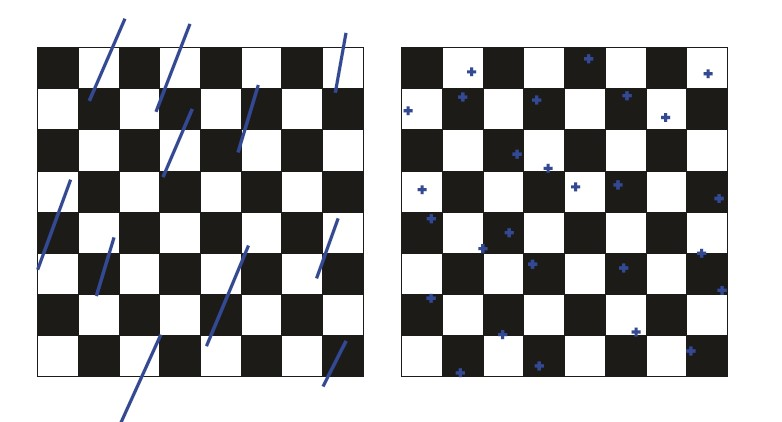
\includegraphics[width=0.5\textwidth]{Imagens/estatisticaDePoison.jpg}
		}%
		\caption{Estatísticas de Poisson. Esta classe de estatísticas pode ser descrita pela “analogia da gota de chuva” conforme mostrado acima. Isso é relevante para a radioterapia, pois a radiação que atinge as células é bastante semelhante a gotas de chuva atingindo uma placa.}
		\label{fig:estatisticaDePoison}
	\end{figure}

	$D_0$ é definido como a dose de radiação que resulta em 37\% de sobrevivência. Supõe-se que essa dose seja igual à dose de radiação necessária para causar um golpe letal por célula.
	
	O modelo de Poisson também é usado para probabilidade de controle de tumor (TCP):

	\begin{itemize}
		\item Em uma média de X células tumorais sobreviventes por paciente:
		\begin{itemize}[label=\textcolor{CarnationPink}{$\star$}]
			\item \textcolor{DarkTurquoise}{\textbf{$\mathbf{\left(e^{-X}\right)}$}}  pacientes são curados (nenhuma célula tumoral);
			\item \textcolor{DarkTurquoise}{\textbf{$\mathbf{\left(1 - e^{-X}\right)}$}} pacientes tiveram recorrência (no mínimo 1 célula tumoral)
		\end{itemize}

		\item Baseado nessa equação temos:
		\begin{itemize}[label=\textcolor{CarnationPink}{$\star$}]
			\item \textcolor{DarkTurquoise}{\textbf{1 célula tumoral por pcte:}} \textbf{TCP = 0.37}
			\item \textcolor{DarkTurquoise}{\textbf{0.5 célula tumoral por pcte:}} \textbf{TCP = 0.61}
			\item \textcolor{DarkTurquoise}{\textbf{0.1 célula tumoral por pcte:}} \textbf{TCP = 0.90}
			\item \textcolor{DarkTurquoise}{\textbf{0.05 célula tumoral por pcte:}} \textbf{TCP = 0.95}
			\item \textcolor{DarkTurquoise}{\textbf{0.01 célula tumoral por pcte:}} \textbf{TCP = 0.99}
		\end{itemize}
		\item \textcolor{DarkTurquoise}{\textbf{Regra prática:}} para atingir um determinado TCP, você deve apontar para uma sobrevivência de células tumorais de (1 - TCP).
	\end{itemize}


\section{Modelo de Alvo Único, Impacto Único}

	O modelo de sobrevivência celular "Single-Target, Single-Hit" (ou Modelo de Alvo Único, Impacto Único) é um modelo simplificado utilizado na radiobiologia para descrever a sobrevivência das células após a irradiação com radiação ionizante. Esse modelo assume que cada célula tem um único alvo crítico (como um núcleo celular) e que se atingido alvo leva à morte da célula.

	No modelo "Single-Target, Single-Hit", a resposta das células à radiação é binária: ou o alvo é atingido e a célula é inativada (morte celular) ou o alvo não é atingido e a célula permanece viva. Portanto, não leva em consideração a possibilidade de danos reparáveis no DNA ou outros efeitos colaterais da radiação.

	Para uma dada dose $\mathcal{D}$: 

	\begin{equation}
		SF(\mathcal{D}) = e^{-\mathcal{D}/D_0}
	\end{equation}

	\begin{exemplo}[onde:]
		\begin{itemize}
			\item \textcolor{DarkTurquoise}{\textbf{$D_0$}} (“D-Zero”) = dose necessária para causar 1 golpe letal por célula
			\item \textcolor{DarkTurquoise}{\textbf{$n$}} = 1.
			\item \textcolor{DarkTurquoise}{\textbf{$D_q$}} = 0.
			\item Quando você plota seus pontos de dados SF versus Dose em um gráfico semilog, seria uma linha reta, indicando que a sobrevivência é uma função exponencial da dose. Ou seja, uma linha reta em um gráfico semilog significa puramente uma morte exponencial que é definida apenas por $D_0$. 
			\item Se $\mathcal{D} = D_0$, $SF(\mathcal{D}) = e^{- D_0/D_0} = e^{-1} = 0.37$ que também é chamado \textcolor{DarkTurquoise}{\textbf{$D_{37}$}}
			\item Este tipo de curva de sobrevivência é visto para células de mamíferos que são irradiadas com radiação de alta LET (densamente ionizante), como partículas alfa ou íons de carbono; células muito sensíveis à radiação, como linfócitos e células da medula óssea; células que apresentam grandes defeitos no reparo da quebra da fita dupla do DNA; células que estão sincronizadas na fase M; e para células que têm reparo de quebra de fita dupla de DNA inibido quimicamente ou por supressão de genes.
		\end{itemize}
	\end{exemplo}

\section{Modelo de Múltiplos Alvos, Hit Único}

	Este modelo assume que cada célula tem vários alvos independentes, todos os quais devem ser atingidos para matar a célula.  O modelo "Multitarget, Single-Hit" (MTSH) é utilizado para descrever a resposta biológica à exposição a radiação de baixa LET, como raios X e raios gama.

	De acordo com o modelo MTSH, uma única partícula de radiação pode causar danos em múltiplos alvos moleculares dentro de uma célula. Isso ocorre porque a radiação ionizante pode liberar elétrons secundários e íons que interagem com as moléculas do meio biológico, causando danos ao DNA e a outras estruturas celulares. Esses danos são chamados de lesões pontuais.  

	No modelo MTSH, cada lesão pontual é considerada um evento independente. Isso significa que a probabilidade de uma lesão pontual ocorrer em um alvo molecular específico é a mesma, independentemente de ocorrerem lesões pontuais em outros alvos. Essa abordagem é uma simplificação, mas é útil para descrever a resposta média de um grande número de células irradiadas.

	A curva do modelo MTSH é apresentada na \ref{fig:singleHitMultiTarget}. Este modelo é importante para entender como a radiação afeta células e tecidos onde é possível estimar os efeitos biológicos da radiação em diferentes doses e taxas de dose. Além disso, o modelo MTSH também é usado para calcular os efeitos de danos cumulativos causados por exposições repetidas à radiação ao longo do tempo.

	\begin{figure}[h]
		\centering
		\fcolorbox{DarkTurquoise}{white}{%
			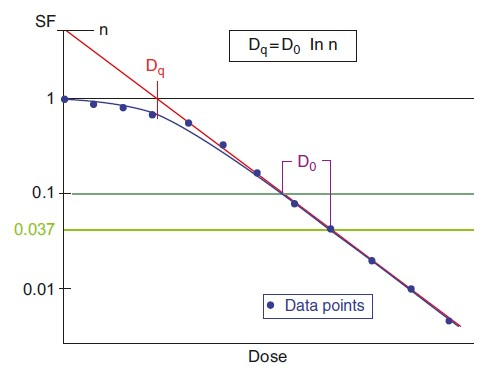
\includegraphics[width=0.8\textwidth]{Imagens/singleHitMultiTarget.jpg}
		}%
		\caption{Curva de sobrevivência de Múltiplos Alvos, Hit Único. Apresenta uma curva em doses baixas e uma reta (por exemplo, a sobrevida é uma função exponencial da dose) em doses altas. Isso permite que seja calculado o $D_0$ fazendo medições na região de alta dose.}
		\label{fig:singleHitMultiTarget}
	\end{figure}

	Para uma única dose $D$:

	\begin{equation}
		SF(D) = 1 - \left(1 - e ^{- \frac{D}{D_0}}\right)^n
	\end{equation}

	\begin{exemplo}[onde,]
		\begin{itemize}
			\item \textcolor{DarkTurquoise}{$\mathbf{D_0}(``D Zero'')$:}  é na dose necessária para causar um impacto por célula;
			\item \textcolor{DarkTurquoise}{$\mathbf{n}$} é o número de extrapolação. É uma medida da largura do ombro. Se n for grande (por exemplo, 10 ou 12), a curva de sobrevivência tem um ombro largo. Se n for pequeno (por exemplo, 1,5 a 2), o ombro da curva é estreito. 
			\item \textcolor{DarkTurquoise}{$\mathbf{D_q = D_0 \times \ln n}$:} é a dose quase-limite -- Outra medida da largura dos ombro. A dose quase limiar é quase uma dose limiar. É definida como a dose na qual a porção reta da curva de sobrevivência, extrapolada para trás, corta o eixo da dose traçado através de uma fração de sobrevivência de unidade. Um limiar de dose é a dose abaixo da qual não há efeito. Não há dose abaixo da qual a radiação não produza nenhum efeito, então não pode haver uma verdadeira dose limite; Dq, a dose quase limite, é a coisa mais próxima.
		\end{itemize}
	\end{exemplo}

	\begin{tcolorbox}[width=\textwidth, colback={white}, colbacktitle={DarkTurquoise!50!white}, title={$\bigstar$ \LobsterTwo{Para entender melhor: Gráfico do Modelo de Múltiplos Alvos, Hit Único } $\bigstar $}, coltitle={CarnationPink}, colframe={DarkTurquoise}, fonttitle=\rmfamily\bfseries\Large]

		Para entender melhor a \ref{fig:singleHitMultiTarget}:
		
		\begin{itemize}
			\item Plotando os pontos de dados de \textcolor{MediumOrchid}{$\mathbf{SF}$} em um gráfico semilog:
			\begin{itemize}[label=\textcolor{CarnationPink}{$\star$}]
				\item \textcolor{MediumOrchid}{$\mathbf{\ln SF}$} estará no eixo logarítmico y;
				\item A dose \textcolor{MediumOrchid}{$\mathbf{D}$} estará no eixo x.
			\end{itemize}
			
			\item Desenhando uma linha reta que conecta todos os pontos de alta dose:
			\begin{itemize}[label=\textcolor{CarnationPink}{$\star$}]
				\item \textcolor{MediumOrchid}{$\mathbf{\ln n}$} será o ponto de interceção no eixo Y.
				\item \textcolor{MediumOrchid}{$\mathbf{D_q}$} será o ponto de interceção no eixo X.
				\item \textcolor{MediumOrchid}{$\mathbf{D_0 = D_q / \ln n}$} é o coeficiente angular da reta. 
			\end{itemize}
		\end{itemize}
	\end{tcolorbox}
	
	

	\begin{itemize}
		\item A porção de alta dose da curva é na verdade uma linha reta:
		
		\begin{itemize}[label=\textcolor{CarnationPink}{$\star$}]
			\item \textcolor{DarkTurquoise}{$\mathbf{D_0}$} é definida como a dose adicional necessária para reduzir a fração de sobrevivência para 37\% da fração de sobrevivência anterior. (\textcolor{MediumOrchid}{\textbf{\LobsterTwo{Obs:}}} Não determine $D_0$ no ponto $SF = 0.37$ caso a curva de sobrevivência tiver um ombro, deve-se lembrar que $D_0$ se aplica à região de alta dose da curva nesse caso! Em vez disso, meça a diferença na dose para os pontos entre $SF = 0.1$ e $SF = 0.037$.)
		
			\item \textcolor{DarkTurquoise}{$\mathbf{D_0}$} é uma medida da radiossensibilidade inerente da célula. A maioria dos valores de $D_0$ está em torno de 1 Gy.
		
			\item \textcolor{DarkTurquoise}{$\mathbf{D_{10} = 2.3 \times D_0}$:} uma dose que reduzirá a fração de sobrevivência em dez vezes (por exemplo, de $SF = 0.1$ para $SF = 0.01$).
		\end{itemize}

		\item A região de baixa dose da curva é conhecida como “ombro”:
		\begin{itemize}[label=\textcolor{CarnationPink}{$\star$}]
			\item \textcolor{DarkTurquoise}{$\mathbf{D_q}$} informa a largura do ombro.
			\item \textcolor{DarkTurquoise}{$\mathbf{D_q}$} é uma medida da capacidade de reparo da célula. Mais reparo significa um $D_q$ maior e um ombro maior.
			\item 
		\end{itemize}

		\item Este tipo de curva de sobrevivência é muito comum para muitas células de mamíferos com reparo de DNA intacto e com resistência intermediária e alta à morte radio-induzida causada por radiações de baixo LET de raios X e raios gama.
	\end{itemize}

	  As principais vantagens desse modelo são:

	  \begin{itemize}
		\item \textcolor{DarkTurquoise}{\textbf{Simplicidade:}} O modelo MTSH é uma abordagem simplificada para descrever os efeitos da radiação, o que facilita sua aplicação e compreensão. Ele considera as lesões pontuais como eventos independentes e não leva em conta fatores mais complexos, como a reparação do DNA e a resposta imune. Essa simplicidade permite a aplicação do modelo em cálculos e estimativas rápidas pois a porção de alta dose da curva é uma linha reta podendo ser desenhada uma com um lápis e uma régua.
		\item \textcolor{DarkTurquoise}{\textbf{Precisão em Altas Doses:}} Esta componente em linha reta se correlaciona bem com experimentos de cultura de células de modo que este modelo é mais preciso para altas doses do que para baixas doses.
		\item \textcolor{DarkTurquoise}{\textbf{Estimativa de danos acumulativo:}} O modelo MTSH é útil para calcular os efeitos cumulativos da radiação ao longo do tempo. Ao considerar cada lesão pontual como um evento independente, é possível estimar a probabilidade de danos cumulativos em um grande número de células irradiadas. Isso é especialmente relevante em exposições repetidas à radiação, como tratamentos de radioterapia fracionada.
	  \end{itemize}

	  As principais desvantagens desse modelo são:

	  \begin{itemize}
		\item \textcolor{DarkTurquoise}{\textbf{Imprecisão em baixas doses:}} A região de baixa dose da curva subestima muito a morte celular.
		\item \textcolor{DarkTurquoise}{\textbf{Não baseia-se em um mecanismo molecular:}} Ao contrário do modelo linear-quadrático, o modelo single-hit não é baseado em um mecanismo molecular. O modelo MTSH é uma simplificação da resposta biológica à radiação e não considera todos os fatores e processos envolvidos. Ele não leva em conta a reparação do DNA, a resposta imune e outros mecanismos de defesa celular. Portanto, pode não refletir completamente a complexidade da resposta biológica real.
		\item \textcolor{DarkTurquoise}{\textbf{Não possui equação simples para a dose equivalente:}} Ao contrário do modelo linear-quadrático, não há uma equação simples para “dose equivalente” dada uma programação diária de fracionamento. 
	  \end{itemize} 


\subsection*{Fracionamento e $D_0$ Efetivo}

	No modelo Multitarget, Single-Hit (MTSH), o fracionamento da dose é um aspecto importante que influencia a curva de sobrevivência celular. O fracionamento da dose refere-se à divisão da dose total em várias frações menores, administradas em momentos diferentes. 

	Após cada fração de radiação, as células têm a oportunidade de se recuperar e reparar os danos causados pela radiação. A eficiência e a velocidade da reparação do DNA podem variar entre diferentes células e tipos de danos. O fracionamento da dose permite que as células reparem parte dos danos entre as frações, resultando em uma maior sobrevivência celular em comparação com uma dose única.

	O fracionamento da dose também pode afetar a disponibilidade de oxigênio nas células tumorais. Durante o intervalo entre as frações, os vasos sanguíneos podem se reperfundir, aumentando a oferta de oxigênio nas áreas irradiadas. Isso pode tornar as células tumorais mais sensíveis à radiação, levando a uma maior eficácia do tratamento.

	Uma curva de sobrevivência para entregas de dose fracionada tem uma inclinação menor em comparação com uma curva de sobrevivência de fração única. Assumindo o reparo completo entre as frações, o ombro é repetido a cada fração, como mostra a \ref{fig:modeloEFracionamento}, onde o coeficiente angular da reta é chamado de $D_0$ efetiva ($D_{0_{eff}}$).

	\begin{figure}[h]
		\centering
		\fcolorbox{DarkTurquoise}{white}{%
			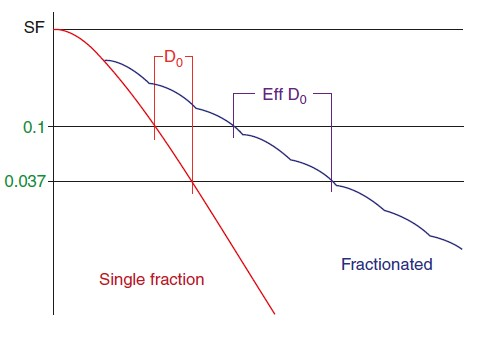
\includegraphics[width=0.7\textwidth]{Imagens/modeloEFracionamento.jpg}
		}%
		\caption{$D_0$ versus $D_{0_{eff}}$. Quando a dose de radiação é fracionada, é necessário muito mais dose para atingir a mesma quantidade de morte celular. Portanto, $D_{0_{eff}}$ é sempre maior que $D_0$.}
		\label{fig:modeloEFracionamento}
	\end{figure}


	Para uma única fração \textcolor{MediumOrchid}{$\mathbf{D \text{ Gy}}$}  com uma fração de sobrevivência de \textcolor{MediumOrchid}{$\mathbf{SF_D}$}:

	\begin{equation}
		D_{0_{eff}} = - \frac{\ln \left(SF_D\right)}{D}
	\end{equation}

	\begin{equation}
		D_{10_{eff}} = - \frac{\log \left(SF_D\right)}{D} = 2.3 \times D_{0_{eff}}
	\end{equation}

	Após \textcolor{MediumOrchid}{\textbf{X}} frações para a dose total \textcolor{MediumOrchid}{$\mathbf{XD \text{ Gy}}$}:

	\begin{equation}
		SF_{XD} = e^{-\frac{XD}{D_{0_{eff}}}}
	\end{equation}

	\textcolor{DarkTurquoise}{\textbf{$\mathbf{D_0}$ efetiva}} é sempre maior que o valor real de \textcolor{MediumOrchid}{$\mathbf{D_0}$}.

	\begin{itemize}[label=\textcolor{CarnationPink}{$\blacktriangleright$}]
		\item \textcolor{MediumOrchid}{\LobsterTwo\textbf{Por Exemplo:}} para $SF_{2Gy} = 0.5$, $D_{0_{eff}} = 2.89 \text{ Gy}$ enquanto um valor típico de $D_0 \sim 1.1 \text{ Gy}$
	\end{itemize}

	\begin{tcolorbox}[width=\textwidth, colback={white}, colbacktitle={DarkTurquoise!50!white}, title={$\bigstar$ \LobsterTwo{Para entender Melhor: Curva de Sobrevivência E Fracionamento} $\bigstar $}, coltitle={CarnationPink}, colframe={DarkTurquoise}, fonttitle=\rmfamily\bfseries\Large]
		
		\begin{itemize}
			\item Primeiro, descubra a resposta para uma pergunta que pede uma fração de sobrevivência \textcolor{MediumOrchid}{$\mathbf{(SF)}$}  ou uma probabilidade de controle do tumor \textcolor{MediumOrchid}{$\mathbf{(TCP)}$}. Considere o seguinte:
			\begin{itemize}[label=\textcolor{CarnationPink}{$\star$}]
				\item “Qual é a dose necessária para matar 99\% das células tumorais?” -- Isso está pedindo um \textcolor{DarkTurquoise}{$\mathbf{SF = 0.01}$};
				\item “Qual é a dose necessária para dar 99\% de controle tumoral de um tumor com $\mathrm{10^9}$ células?” -- Isso está pedindo um \textcolor{MediumOrchid}{$\mathbf{TCP = 0.99}$} que equivale a 0.01 células tumorais de modo que \textcolor{DarkTurquoise}{$\mathbf{SF = 0.01/10^9 = 10^{-11}}$}
			\end{itemize}
			\item Em seguida, descubra uma \textcolor{DarkTurquoise}{$\mathbf{D_{0_{eff}} = \ln (SF)/D_0}$}
			\item A \textcolor{DarkTurquoise}{$\mathbf{D_{10_{eff}}}$} $2.3 \times D_{0_{eff}}$, onde cada \textcolor{MediumOrchid}{$\mathbf{D_{10}}$} efetiva reduzirá a \textcolor{MediumOrchid}{$\mathbf{SF}$} em dez vezes:
			\begin{itemize}[label=\textcolor{CarnationPink}{$\star$}]
				\item Para alcançar uma $SF = 0.01$ a dose total $D_{tot} = 2 \times D_{10_{eff}}$
				\item Para alcançar uma $SF = 10^{-11}$ a dose total $D_{tot} = 11 \times D_{10_{eff}}$
			\end{itemize}
		\end{itemize}

	\end{tcolorbox}
	
\section{Modelo Linear-Quadrático (LQ, Alfa-Beta)}

	O modelo linear-quadrático (LQ) é um dos modelos mais amplamente utilizados na radiobiologia para descrever a resposta biológica à radiação ionizante. Ele leva em consideração a relação entre a dose de radiação e o efeito biológico, levando em conta tanto os danos diretos quanto os danos indiretos causados pela radiação.

	O modelo LQ é baseado na suposição de que os danos biológicos resultam de dois tipos de eventos: danos lineares proporcionais à dose e danos quadráticos proporcionais ao quadrado da dose. Em outras palavras, o modelo assume que a resposta biológica é uma combinação de efeitos lineares e quadráticos da dose.

	O modelo linear-quadrático foi desenvolvido após a observação in vitro de que o dano ao DNA segue uma relação linear-quadrática com a dose D, como mostra a \ref{fig:modeloLinearQuadratico2}. Nesse modelo, a quantidade de aberrações letais no DNA causando a morte celular é  igual a $\alpha D + \beta D^2$ 

	\begin{figure}[h]
		\centering
		\fcolorbox{DarkTurquoise}{white}{%
			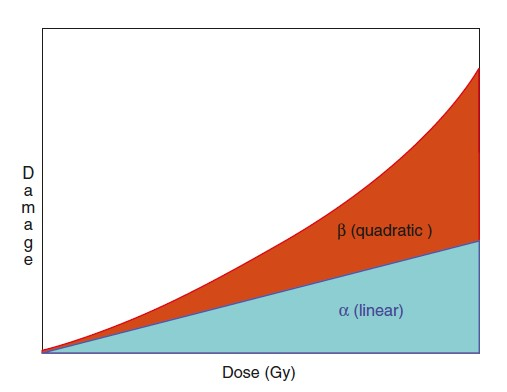
\includegraphics[width=0.6\textwidth]{Imagens/modeloLinearQuadratico.jpg}
		}%
		\caption{A curva linear-quadrática de danos ao DNA. O dano total ao DNA pode ser expresso como a soma do dano “linear” (não dependente do tamanho da fração) e “quadrático” (dependente do tamanho da fração).}
		\label{fig:modeloLinearQuadratico2}
	\end{figure}

	A fração de sobrevivência para uma dada dose $D$ é dada por:

	\begin{equation}
		SF_{D} = e^{- \left(\alpha D + \beta D^2\right)}
	\end{equation}

	\begin{exemplo}[onde,]
		\begin{itemize}
			\item \textcolor{DarkTurquoise}{$\mathbf{SF_D}$} é a fração de sobrevivência celular, representando a proporção de células que permanecem viáveis após a exposição à radiação.
			\item \textcolor{DarkTurquoise}{$\mathbf{D}$} é a dose de radiação administrada.
			\item \textcolor{DarkTurquoise}{$\mathbf{\alpha}$} é o coeficiente linear de danos, que representa a taxa na qual as células são danificadas de forma linear em relação à dose.
			\item \textcolor{DarkTurquoise}{$\mathbf{\beta}$} é o coeficiente quadrático de danos, que representa a taxa na qual as células são danificadas de forma quadrática em relação à dose.
		\end{itemize}
	\end{exemplo}

	Ao contrário do modelo single-hit, o modelo LQ é responsável por dois tipos diferentes de hits (golpes) letais que são baseados em mecanismos moleculares conhecidos de dano ao DNA:
	
	\begin{itemize}[label=\textcolor{CarnationPink}{$\blacktriangleright$}]
		\item \textcolor{DarkTurquoise}{\textbf{Morte com um único golpe ($\alpha$)}} é um dano irreparável e é independente de fracionamento ou taxa de dose que corresponde golpe único e dano acumulado intra-track.
		\item \textcolor{DarkTurquoise}{\textbf{Morte com dois golpes ($\beta$)}} é um dano reparável e depende de fracionamento e taxa de dose que corresponde ao dano acumulado inter-track.
	\end{itemize}

	Quando dizemos que um dano é linear com a dose, significa que o efeito biológico causado pela radiação é proporcional à quantidade de radiação absorvida. Em outras palavras, quanto maior a dose de radiação, maior será o dano biológico causado. Esse dano linear é representado pelo termo $\alpha$ na equação do modelo linear-quadrático.

	Por exemplo, suponha que uma célula seja exposta a uma determinada dose de radiação. Se o dano for linear com a dose, ao dobrarmos a dose, o dano também será duplicado. Da mesma forma, se reduzirmos a dose pela metade, o dano será reduzido pela metade.

	Já quando um dano é quadrático com a dose, significa que o efeito biológico não é apenas proporcional à dose, mas também é influenciado pelo quadrado da dose. Isso significa que um aumento na dose resultará em um aumento não apenas proporcional, mas também exponencial no dano biológico. Esse dano quadrático é representado pelo termo $\beta$ na equação do modelo linear-quadrático.

	Por exemplo, se dobrarmos a dose de radiação quando o dano é quadrático, o dano biológico não será apenas dobrado, mas será aumentado em um fator muito maior devido ao efeito quadrático. Da mesma forma, uma redução na dose pela metade levará a uma redução muito maior do dano biológico.

	Portanto, danos lineares com a dose significam que o efeito biológico aumenta proporcionalmente à dose de radiação, enquanto danos quadráticos com a dose significam que o efeito biológico aumenta de forma exponencial à dose de radiação, levando a um aumento mais acentuado nos efeitos biológicos.



	É importante observar que, a curva para a fração de sobrevivência é a mesma para os modelos, porém cada modelo aborda diferentes métodos para explicar a forma da curva. A \ref{fracaoSobrevivencia} mostra uma comparação dos parâmetros utilizados no modelo multi-alvos e o modelo linear quadrático.

	\begin{figure}[h]
		\centering
		\fcolorbox{DarkTurquoise}{white}{%
			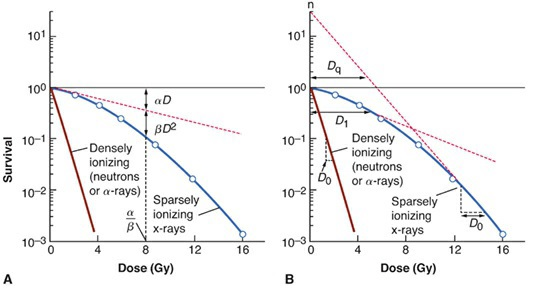
\includegraphics[width=0.6\textwidth]{Imagens/fracaoSobrevivencia.jpg}
		}%
		\caption{Forma da curva de sobrevivência para células de mamíferos expostas à radiação. A fração de células sobreviventes é plotada em uma escala logarítmica contra a dose em uma escala linear. Para partículas alfa ou nêutrons de baixa energia (denominados densamente ionizantes), a curva dose-resposta é uma linha reta desde a origem (ou seja, a sobrevivência é uma função exponencial da dose). A curva de sobrevivência pode ser descrita por apenas um parâmetro, a inclinação. Para os raios x ou gama (ditos como pouco ionizantes), a curva dose-resposta tem uma inclinação linear inicial, seguida por um ombro; em doses mais altas, a curva tende a ficar reta novamente. \textbf{A:} O modelo linear quadrático. Os dados experimentais são ajustados a uma função linear-quadrática. Existem dois componentes da morte celular: um é proporcional à dose 
		$(\alpha D)$; o outro é proporcional ao quadrado da dose $(\beta D^2)$. A dose na qual os componentes linear e quadrático são iguais é a razão $\alpha/\beta$. A curva linear-quadrática se curva continuamente, mas é um bom ajuste para dados experimentais para as primeiras décadas de sobrevivência. \textbf{B:} O modelo multialvo. A curva é descrita pela inclinação inicial $(D_1)$, a inclinação final $(D_0)$ e um parâmetro que representa a largura do ombro, seja $n$ ou $D_q$.}
		\label{fig:fracaoSobrevivencia}
	\end{figure}

	No modelo linear quadrático, Os componentes da morte celular que são proporcionais à dose e ao quadrado da dose são iguais se:

	\begin{equation}
		\alpha D = \beta D^2
	\end{equation}

	ou

	\begin{equation}
		D = \frac{\alpha}{\beta}
	\end{equation}

	Ou seja, as contribuições linear e quadrática para a morte celular são iguais em uma dose que é igual à proporção de $\alpha$ para $\beta$:

	\begin{itemize}
		\item \textcolor{DarkTurquoise}{\textbf{Baixa razão $\alpha/\beta$  (“alto reparo”)}} os tecidos são relativamente resistentes em pequenas frações e relativamente sensíveis em grandes frações.
		\item \textcolor{DarkTurquoise}{\textbf{Alta razão $\alpha/\beta$ (“baixo reparo”)}} os tecidos são relativamente sensíveis em pequenas frações e relativamente resistentes em grandes frações.
	\end{itemize}


\section{Taxa de Dose}

	A morte de células de mamíferos radio-induzida pela radiação de baixa LET tem uma forte dependência com a taxa de dose abaixo de 1Gy/minuto e geralmente o "efeito da taxa de dose" é observado entre 1 e 100 cGy/min em várias linhagens de células de mamíferos. À medida que a taxa de dose é reduzida, para a radiação de baixa LET, a morte de células de mamíferos é reduzida e a curva de sobrevivência torna-se mais rasa ($D_0$ aumenta) e o ombro tende a desaparecer.

	A dependência da morte de células de mamíferos radio-induzida pela radiação de baixa LET (Linear Energy Transfer) com a taxa de dose segue um padrão geralmente chamado de "lei da taxa química de ação". De acordo com essa lei, a fração de células sobreviventes diminui de forma exponencial com o aumento da taxa de dose. 

	Em outras palavras, à medida que a taxa de dose aumenta, a fração de células que sobrevivem à radiação diminui de forma mais rápida. Isso significa que, para uma mesma dose total de radiação de baixa LET, quando a taxa de dose é alta, menos células sobrevivem em comparação com uma taxa de dose mais baixa.

	A lei da taxa química de ação é uma simplificação que assume uma dependência exponencial inversa entre a taxa de dose e a sobrevivência celular. No entanto, é importante ressaltar que a resposta biológica real pode ser mais complexa, e outros fatores, como a sensibilidade específica das células e as vias de reparação do DNA, podem influenciar a curva de sobrevivência celular.

	As células radio-resistentes com ombros largos em suas curvas de sobrevivência têm grandes efeitos poupadores de taxa de dose. Por outro lado, células de mamíferos sensíveis à radiação e células com defeitos de reparo de DNA DSB que têm curvas de sobrevivência quase puramente exponenciais, com muito pouca evidência de um ombro têm muito pouca ou nenhuma efeito poupador ao diminuir as taxas de dose abaixo de 1 Gy/minuto (\ref{fig:efeitoTaxaDeDose}).

	\begin{figure}[h]
		\centering
		\fcolorbox{DarkTurquoise}{white}{%
			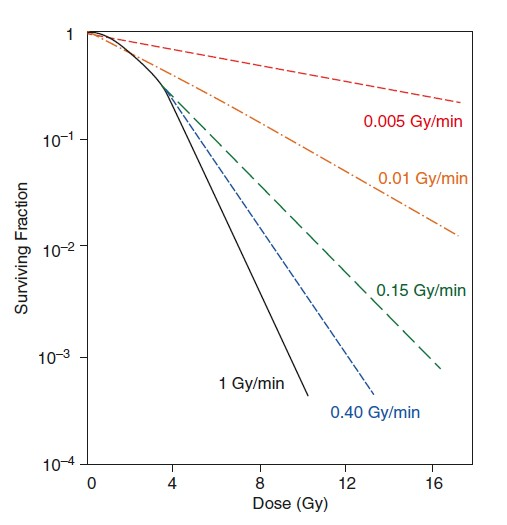
\includegraphics[width=0.5\textwidth]{Imagens/efeitoTaxaDeDose.jpg}
		}%
		\caption{O efeito da taxa de dose inferior a 1 Gy/min em uma curva de sobrevivência de células de mamíferos com um ombro indicativo de resistência à radiação. Abaixo de 1 Gy/min acaba poupando significativamente a morte celular radio-induzida por radiação de baixa LET, e resulta em uma maior sobrevivência em um achatamento da inclinação da curva de sobrevivência devido ao reparo do DNA que ocorre durante o período de irradiação para fornecer várias doses em Gy.}
		\label{fig:efeitoTaxaDeDose}
	\end{figure}

	A morte de células de mamíferos radio-induzida pela radiação de alta LET tem muito pouco, se houver, efeito de taxa de dose devido à complexidade do dano ao DNA produzido e à dificuldade de reparar esse dano pelas vias de reparo de danos ao DNA das célula de mamíferos.

	A dependência da morte de células de mamíferos radio-induzida pela radiação de alta LET (Linear Energy Transfer) com a taxa de dose é diferente em comparação com a radiação de baixa LET. A resposta biológica à radiação de alta LET exibe um padrão conhecido como "efeito de saturação".

	Ao contrário da radiação de baixa LET, onde a taxa de dose mais alta resulta em uma diminuição exponencial da sobrevivência celular, a resposta à radiação de alta LET mostra um efeito de saturação. Isso significa que, para doses de radiação de alta LET muito altas, a fração de células que morrem atinge um platô e não diminui significativamente com o aumento da taxa de dose.

	A principal razão por trás desse efeito de saturação é que a radiação de alta LET deposita energia de forma mais concentrada e causa danos mais severos e complexos no DNA das células. Quando a dose de radiação de alta LET é muito alta, os danos são tão extensos que a probabilidade de sobrevivência celular já é bastante baixa, independentemente da taxa de dose.

	É válido destacar também que a dependência da morte celular pela radiação de baixa LET e alta LET com a taxa de dose pode ser diferente em diferentes tipos de células e tecidos. Além disso, a dependência da taxa de dose pode ser modificada por outros fatores, como o tipo de célula, a sensibilidade intrínseca à radiação, a presença de oxigênio (oxygen enhancement ratio) e a capacidade de reparação do DNA.

\subsection*{Ultrahigh Dose Rate (FLASH-RT)}

	A Ultrahigh Dose Rate (FLASH-RT) é uma abordagem inovadora na radioterapia que envolve a administração de doses muito altas de radiação em uma taxa de dose extremamente rápida, em comparação com as técnicas tradicionais de radioterapia. No FLASH-RT, a dose de radiação é entregue em frações de tempo muito curtas, geralmente em menos de 1 segundo, em contraste com as técnicas convencionais que levam vários minutos para administrar a mesma dose.

	A alta taxa de dose característica da FLASH-RT é alcançada por meio do uso de tecnologias avançadas, como aceleradores de partículas de alta potência ou fontes de radiação de intensidade ultrarrápida. Essas tecnologias permitem a liberação rápida e precisa da dose de radiação, o que pode levar a uma exposição temporalmente mais curta dos tecidos normais aos efeitos danosos da radiação. Os aceleradores foram desenvolvidos em meados do século XX, capazes de fornecer doses de elétrons de baixo LET para células e tecidos em pulsos únicos de nanossegundos.

	Nos últimos anos, os investigadores começaram a reinvestigar taxas de dose ultra-altas (100–500 Gy/s) ou em pulsos únicos de nanossegundos agora chamados (FLASH-RT) e realmente encontraram a preservação de tecidos normais no cérebro, abdômen e pele para elétrons, raios X e prótons. Embora a compreensão dos mecanismos subjacentes ao efeito FLASH ainda esteja em evolução, há evidências de que a rápida liberação da dose de radiação leva a respostas biológicas distintas, como uma menor proliferação de células endoteliais e inflamação reduzida em comparação com a radioterapia convencional. 

	O objetivo da FLASH-RT é aproveitar a diferença na resposta biológica das células normais e das células tumorais à radiação administrada em altas taxas de dose. Essas taxas de dose ultra-altas foram utilizadas para estudar a natureza e a cinética do dano e reparo do DNA induzido pela radiação, e o papel do oxigênio no efeito direto versus indireto no dano ao DNA induzido pela radiação e na morte celular em células e tecidos. Vários estudos experimentais em modelos pré-clínicos demonstraram que a radiação entregue em altas taxas de dose, no regime FLASH, pode preservar os tecidos normais, reduzindo a toxicidade aguda e tardia associada à radioterapia convencional, enquanto ainda controla efetivamente o tumor. 

	Os pesquisadores descobriram que se o nível de oxigênio dissolvido fosse baixo o suficiente nas células ou tecidos sendo irradiados (na ordem de alguns por cento), seria possível esgotar todo o oxigênio nas células ou tecidos sendo irradiados e obter apenas dano de DNA de efeito direto (ou seja, 2/3 menos danos ao DNA) por dose física e, portanto, resultaria em menos morte celular ou dano tecidual. Estudos preliminares indicam que os tumores experimentais não são poupados quando irradiados com doses ultra-altas de FLASH-RT e, portanto, esta abordagem tem o potencial de melhorar a relação terapêutica.
	
	A pesquisa em FLASH-RT ainda está em estágios iniciais, mas os resultados iniciais são promissores e levantam a possibilidade de uma radioterapia mais eficaz e segura. No entanto, mais estudos são necessários para entender completamente os efeitos biológicos, os mecanismos subjacentes e a segurança dessa abordagem antes que ela possa ser amplamente adotada na prática clínica.
	
\bibliography{ref.bib}
\end{document}